\documentclass[english,notitlepage]{revtex4-1}  % defines the basic parameters of the document
%For preview: skriv i terminal: latexmk -pdf -pvc filnavn



% if you want a single-column, remove reprint

% allows special characters (including æøå)
\usepackage[utf8]{inputenc}
%\usepackage[english]{babel}

%% note that you may need to download some of these packages manually, it depends on your setup.
%% I recommend downloading TeXMaker, because it includes a large library of the most common packages.

\usepackage{physics,amssymb}  % mathematical symbols (physics imports amsmath)
\include{amsmath}
\usepackage{graphicx}         % include graphics such as plots
\usepackage{xcolor}           % set colors
\usepackage{hyperref}         % automagic cross-referencing (this is GODLIKE)
\usepackage{listings}         % display code
\usepackage{subfigure}        % imports a lot of cool and useful figure commands
\usepackage{float}
%\usepackage[section]{placeins}
\usepackage{algorithm}
\usepackage[noend]{algpseudocode}
\usepackage{subfigure}
\usepackage{tikz}
\usetikzlibrary{quantikz}
% defines the color of hyperref objects
% Blending two colors:  blue!80!black  =  80% blue and 20% black
\hypersetup{ % this is just my personal choice, feel free to change things
    colorlinks,
    linkcolor={red!50!black},
    citecolor={blue!50!black},
    urlcolor={blue!80!black}}

%% Defines the style of the programming listing
%% This is actually my personal template, go ahead and change stuff if you want



%% USEFUL LINKS:
%%
%%   UiO LaTeX guides:        https://www.mn.uio.no/ifi/tjenester/it/hjelp/latex/
%%   mathematics:             https://en.wikibooks.org/wiki/LaTeX/Mathematics

%%   PHYSICS !                https://mirror.hmc.edu/ctan/macros/latex/contrib/physics/physics.pdf

%%   the basics of Tikz:       https://en.wikibooks.org/wiki/LaTeX/PGF/Tikz
%%   all the colors!:          https://en.wikibooks.org/wiki/LaTeX/Colors
%%   how to draw tables:       https://en.wikibooks.org/wiki/LaTeX/Tables
%%   code listing styles:      https://en.wikibooks.org/wiki/LaTeX/Source_Code_Listings
%%   \includegraphics          https://en.wikibooks.org/wiki/LaTeX/Importing_Graphics
%%   learn more about figures  https://en.wikibooks.org/wiki/LaTeX/Floats,_Figures_and_Captions
%%   automagic bibliography:   https://en.wikibooks.org/wiki/LaTeX/Bibliography_Management  (this one is kinda difficult the first time)
%%   REVTeX Guide:             http://www.physics.csbsju.edu/370/papers/Journal_Style_Manuals/auguide4-1.pdf
%%
%%   (this document is of class "revtex4-1", the REVTeX Guide explains how the class works)


%% CREATING THE .pdf FILE USING LINUX IN THE TERMINAL
%%
%% [terminal]$ pdflatex template.tex
%%
%% Run the command twice, always.
%% If you want to use \footnote, you need to run these commands (IN THIS SPECIFIC ORDER)
%%
%% [terminal]$ pdflatex template.tex
%% [terminal]$ bibtex template
%% [terminal]$ pdflatex template.tex
%% [terminal]$ pdflatex template.tex
%%
%% Don't ask me why, I don't know.

\begin{document}

\title{FYS3150 - project 1}      % self-explanatory
\author{Sverre Wehn Noremsaune \& Frida Marie Engøy Westby}          % self-explanatory
\date{\today}                             % self-explanatory
\noaffiliation                            % ignore this, but keep it.


\maketitle 

\begin{center}
	\url{https://github.uio.no/comPhys/FYS3150/tree/project1}
\end{center}

    
\section*{Problem 1}

%\subsection*{Problem a}
We have the one-dimensional Poisson equation
\begin{equation}\label{eq:one-dimensional Poisson}
    - \frac{d^2u}{dx^2} = f(x)
\end{equation}
where $f(x)$ is known to be $100e^{-10x}$. We also assume $x \in [0,1]$, that the boundary condition are $u(0) = 0 = u(1)$ and $u(x)$ is

\begin{equation}\label{eq:exact solution one-dimensional Poisson}
    u(x) = 1 - (1 - e^{-10})x-e^{-10x}
\end{equation}
where $u(x)$ is an exact solution to Eq. (1). We can check this analytically by differentiating $u(x)$ twice.
\begin{equation*}
    \begin{split}
    	-u''(x) &= f(x) \\
    	u''(x) &= -f(x) \\
        u(x)' &= 10x^{-10x} - 1 + \frac{1}{e} \\
        u''(x) &= -100e^{-10x}= -f(x) \quad \blacksquare
    \end{split}
\end{equation*}


%\subsection*{Problem b}
%Write a solution for problem 1b here.
\section*{Problem 2}
	See FIG 1. wich shows the plot of the exact Poisson solution. See 'poisson\_exact.cpp' and 'algorithms.cpp' in the github repository, for source code.
	\begin{figure}[H]
		\centering
		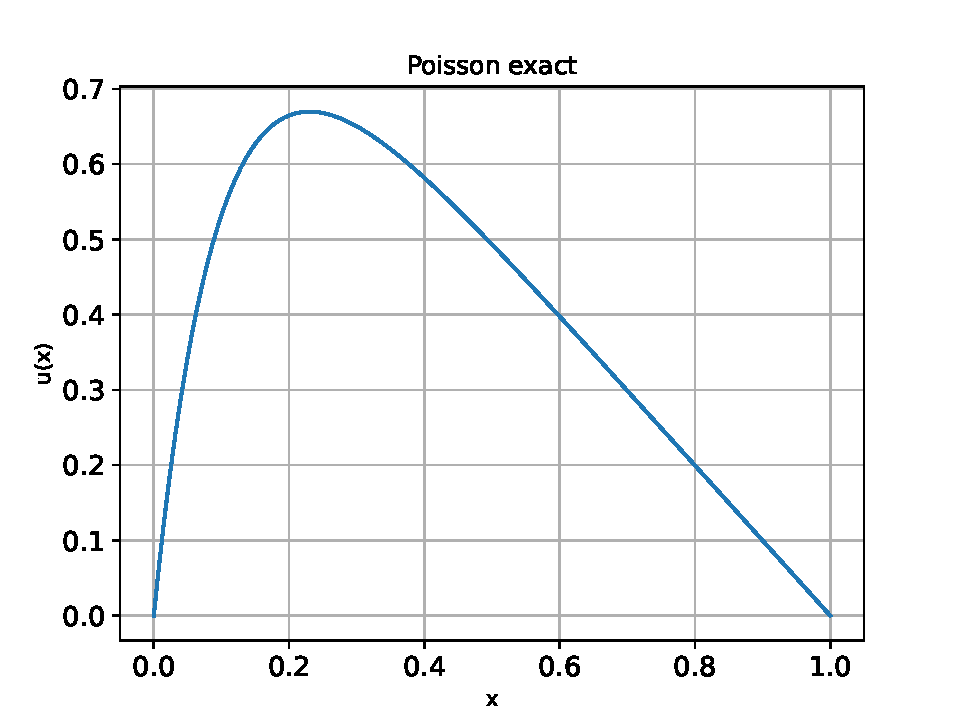
\includegraphics[scale=0.55]{plots/poisson_exact.pdf} %Imports the figure.
		\caption{A plot of the exact solution for the Poisson equation from \ref{eq:one-dimensional Poisson} for $x \in[0,1]$}
		\label{fig:Exact poisson}
	\end{figure}


\section*{problem 3}
	We are discretizing the Poisson equation from \ref{eq:one-dimensional Poisson}.

	Discretizing x and setting up some notation:
	\begin{equation*}
		\begin{split}
			x &\rightarrow x_i \\
			u(x) &\rightarrow u_i \\
			i &= 0,1,\dots,n \\
			h &= \frac{x_{max} - x_{min}}{n} \\
			x_i &= x_0 + ih 
		\end{split}
	\end{equation*}

Next we're using the three-point formula to find the second derivative: \\

\begin{equation*}
 	\frac{du^2}{dx^2} = u'' = \frac{u_{i-1} -2 u_i + u_{i+1}}{h^2} + O(h^2)
\end{equation*}

\begin{equation*}
	f_i = -\left(\frac{u_{i-1} - 2u_i + u_{i+1}}{h^2} + O(h^2)\right)
\end{equation*}

Then we approximate and change the notation, $v_i \approx u_i$ and get

\begin{equation}\label{eq:discretized Poisson}
	f_i = \frac{-v_{i-1} +2 v_i - v_{i+1}}{h^2} \\
\end{equation}


\section*{Problem 4}
The equation we got in \ref{eq:discretized Poisson} isn't the most ergonomic for setting up a matrix equation, so we can rewrite it to
\begin{equation}\label{eq:discretized Poisson 2}
	-v_{i-1} + 2v_i - v_{i+1} = h^2f_i
\end{equation}
Equation \ref{eq:discretized Poisson 2} is a set of equations for every i
$$
\begin{matrix}
	i=1 \quad & -v_0 & 2v_1 & -v_2  &       & = h^2f_i \\
	i=2 \quad &      & -v_1 &  2v_2 & - v_3 & = h^2f_2 \\
\end{matrix}
$$
and so on and so forth. We can see that $v_0$ and $v_n$ will end up and alone on their columns, and since we know what they are we simply move them over. \\
$$
\begin{matrix}
	i=1 \quad  & 2v_1 & -v_2  &       & \quad \quad = h^2f_1 + v_0 \\
	i=2 \quad  & -v_1 &  2v_2 & - v_3 & = h^2f_2 \\
\end{matrix}
$$
This can then be easily rewritten as a matrix equation $A\vec{v} = \vec{g}$
$$
\begin{bmatrix}
	2  & -1 & 0  & 0  & \dots & 0 & 0 & \\
	-1 &  2 & -1 & 0  & \dots & 0 & 0 \\
	0  & -1 & 2  & -1 & \dots & 0 & 0 \\
	\vdots & \vdots & \ddots & \ddots & \ddots & \vdots & \vdots \\
	0 & 0 & \dots &-1 & 2 & -1 & 0 \\
	0 & 0 & \dots & 0 & -1 & 2  & -1 \\
	0 & 0 & \dots & 0 & 0 & -1 & 2
	
\end{bmatrix}
\begin{bmatrix}
	v_1 \\ v_2 \\ v_3 \\ \vdots \\ v_{n-3} \\v_{n-2} \\ v_{n-1}
\end{bmatrix}
=
\begin{bmatrix}
	g_1 \\ g_2 \\ g_3 \\ \vdots \\ g{n-3} \\ g{n-2} \\ g_{n-1}
\end{bmatrix}
$$
where $g_i$ is $h^2f_i$ ($+v_0$ for $f_1$ and $+v_n$ for $f_{n-1}$).


\section*{Problem 5}
\subsection*{Problem a}
We can see that n is related to m since we're "dropping" 2 columns, which gives $n = m-2$

\subsection*{Problem b}
We will find $\vec{{v_i^*}}$ for $1..(n-1)$, meaning everything but the boundary points.


\subsection*{problem 6}
Here will we look at a general tridiagonal matrix, and not the Poisson equation from earlier.

\subsection*{Problem a}
\begin{algorithm}[H]
	\caption{Algorithm for solving general tridiagonal matrix}
	\begin{algorithmic}
		\State arrays a, b, c, u, f, temp of length n
		\\
		\State btemp = b[1]
		\State u[1] = f[1]/btemp
		\\
		\For{ i = 2,3,...,n }
			\State temp[i] = c[i-1] / btemp
			\State btemp = b[i] - a[i] * temp[i]
			\State u[i] = (f[i] - a[i] * u[i-1]) / btemp
		\EndFor
		\For{i = n-1, n-2, ..., 1}
			\State u[i] -= temp[i+1] * u[i+1]
		\EndFor
	\end{algorithmic}
\end{algorithm}

\subsection*{Problem b}
When we analyse the algorithm above, we can see that we get $1 + 6(n-1) + 2(n-1) = 1 + 8(n-1) = 8n - 7$ FLOPs.


\section*{problem 7}
In this problem and the problems below, will we once again look at the Poisson Equation.

\subsection*{Problem a}
See 'general\_tridiag.cpp' and 'algorithms.cpp' in the github repository for the program that solves the Poisson equation with the general algorithm.

\subsection*{Problem b}
	\begin{figure}[H]
	\centering
	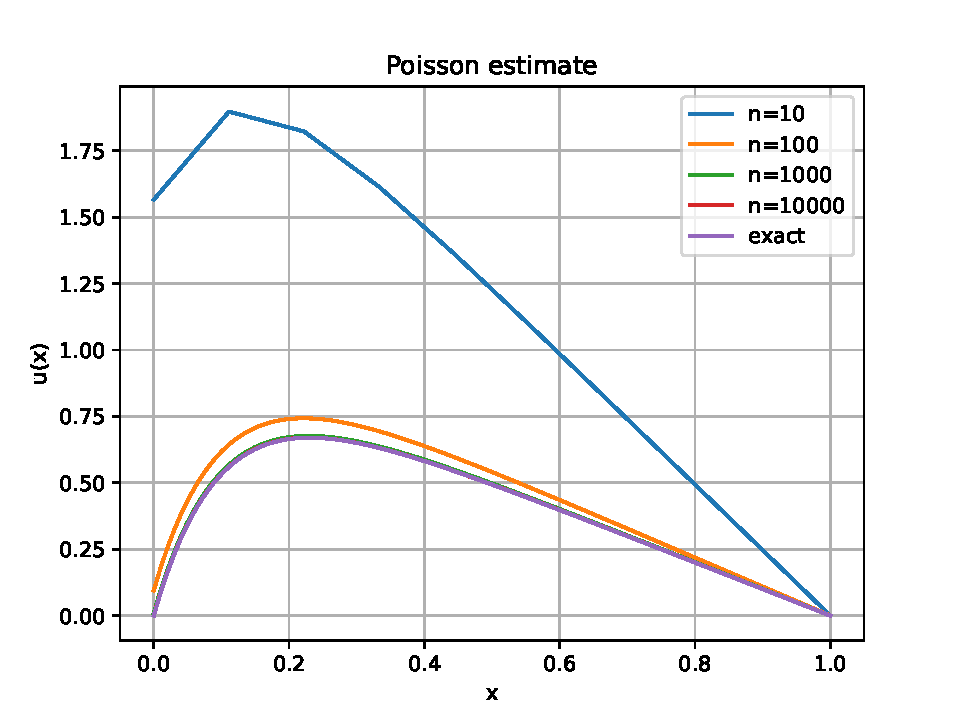
\includegraphics[scale=0.55]{plots/gen_tri_cmp_exact.pdf} %Imports the figure.
	\caption{Exact vs numerical comparison for the solution of equation \ref{eq:one-dimensional Poisson}}
	\label{fig:Exact vs approx Poisson }
	\end{figure}


\section*{problem 8}

	\subsection*{Problem a}
	See FIG 3 for the polt showing the (logarithm of) the absolute error.
		\begin{figure}[H]
			\centering
			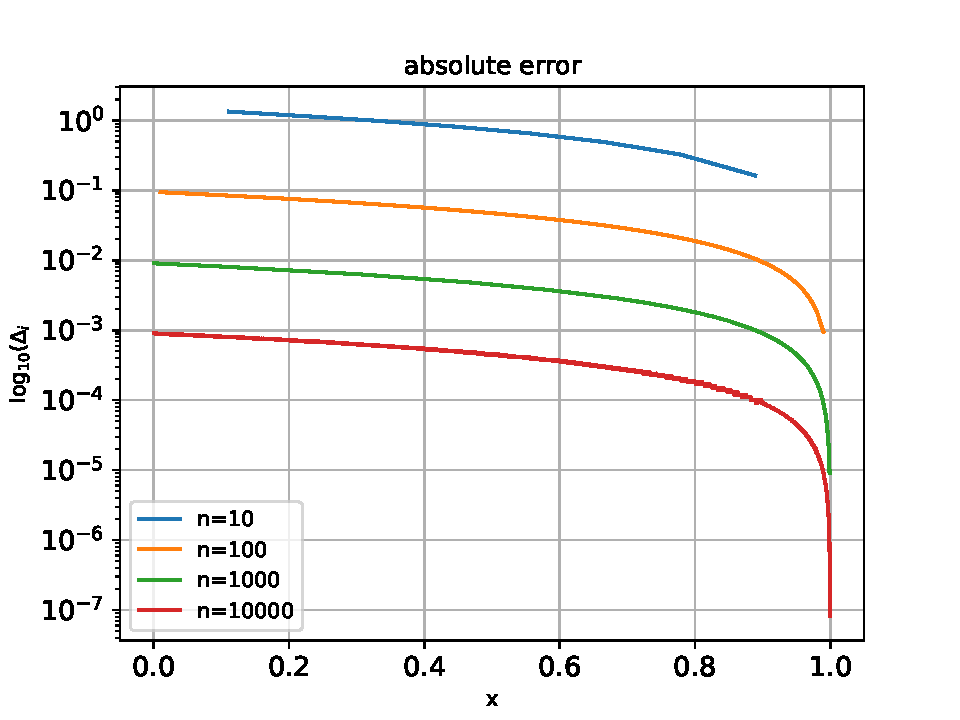
\includegraphics[scale=0.55]{plots/absolute_error.pdf} %Imports the figure.
			\caption{The absolute error for the general tridiagonal alogrithm in $log_{10}$}
			\label{fig:absolute_error}
		\end{figure}

	\subsection*{Problem b}
	See FIG 4 for the polt showing the (logarithm of) the relative error.
		\begin{figure}[H]
			\centering
			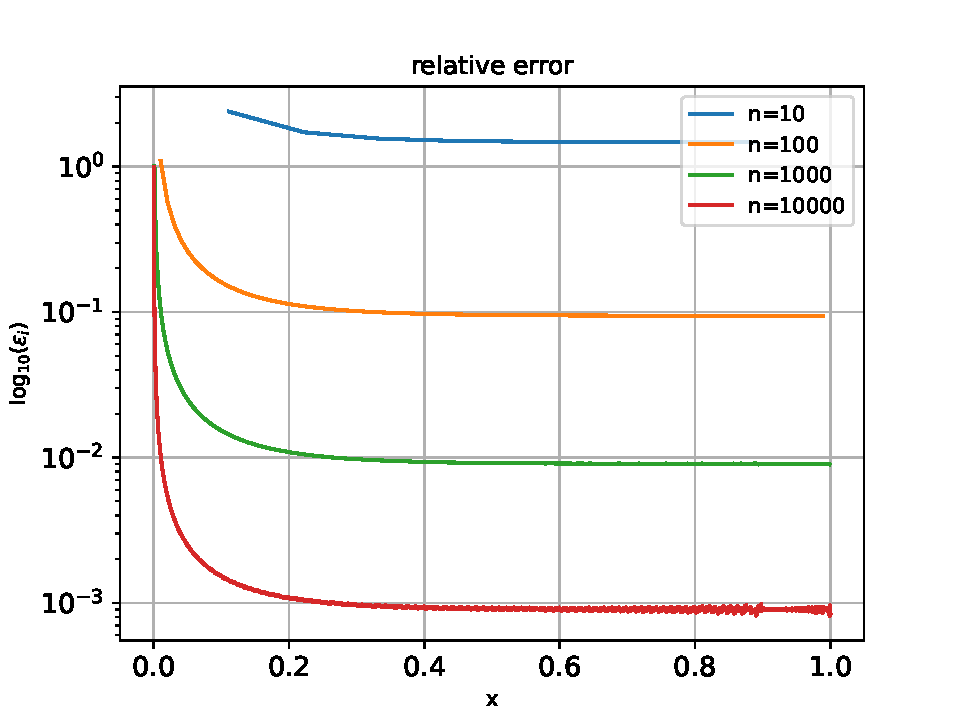
\includegraphics[scale=0.55]{plots/relative_error.pdf} %Imports the figure.
			\caption{The relative error of the general tridiagonal algorithm}
			\label{fig:relative_error}
		\end{figure}

	\subsection*{Problem c}
	See FIG 5 for the plot for the table showing the maximum relative error. We see that for highter $n$ the closer we get to 1.0, and from $n = 1 000 000$ the max relative error becomes 1.0. Combined with the plot of the relative error above, we can see that the approximate and exact value differs quite dramatically close to $x=0$ in comparison to the rest.
		\begin{figure}[H]
			\centering
			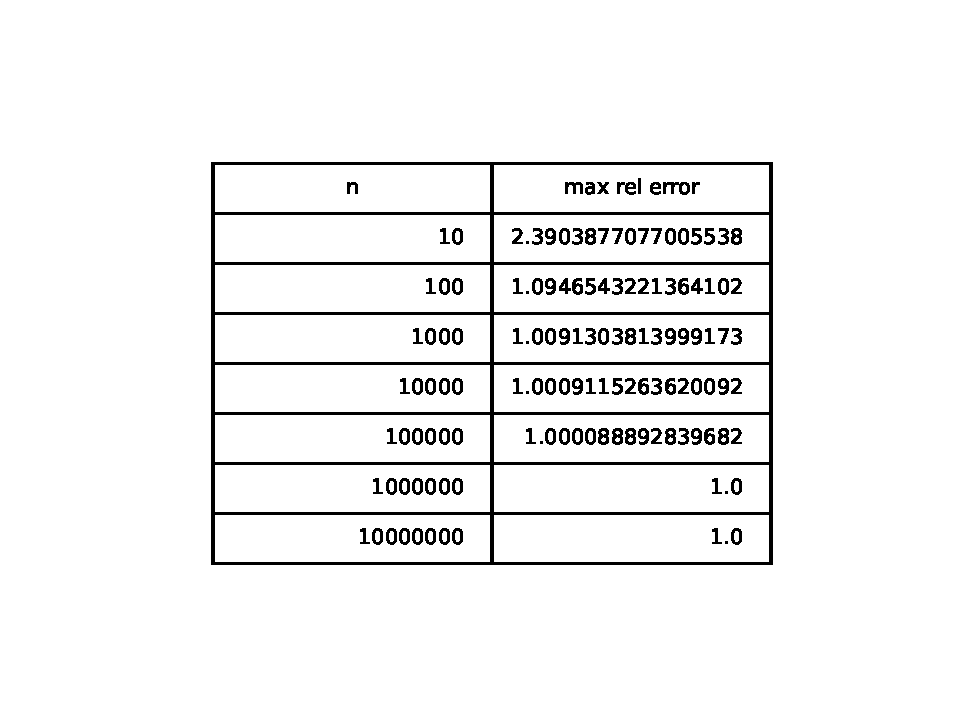
\includegraphics[scale=0.75]{plots/biggest_rel_err.pdf} %Imports the figure.
			\caption{Table with the biggest relative error for each iteration}
			\label{fig:biggest_rel_err}
		\end{figure}


\section*{problem 9}
	Since the values of $a,b,c$ never changes, we can just replace the arrays with a constant, saving us from repeatedly calculating $- (-1)\cdot{something}$.
	\subsection*{Problem a}
		\begin{algorithm}[H]
			\caption{Algorithm for solving special tridiagonal matrix}
			\begin{algorithmic}
				\State arrays u, f, temp of length n
				\\
				\State btemp = 2
				\State u[1] = f[1]/ 2
				\\
				\For{ i = 2,3,...,n }
				\State temp[i] = -1 / btemp
				\State btemp = b[i] + temp[i]
				\State u[i] = (f[i] + u[i-1]) / btemp
				\EndFor
				\For{i = n-1, n-2, ..., 1}
				\State u[i] -= temp[i+1] * u[i+1]
				\EndFor
			\end{algorithmic}
		\end{algorithm}
	\subsection*{Problem b}
		FLOPs: $1 + 4(n-1) + 2(n-1) = 1 + 6(n-1) = 6n - 5$
	\subsection*{Problem c}
	See the function 'special\_tridiag' in 'data\_algorithms.cpp' in the github repository for the special algorithm.



\section*{problem 10}
	\begin{figure}[H]
		\centering
		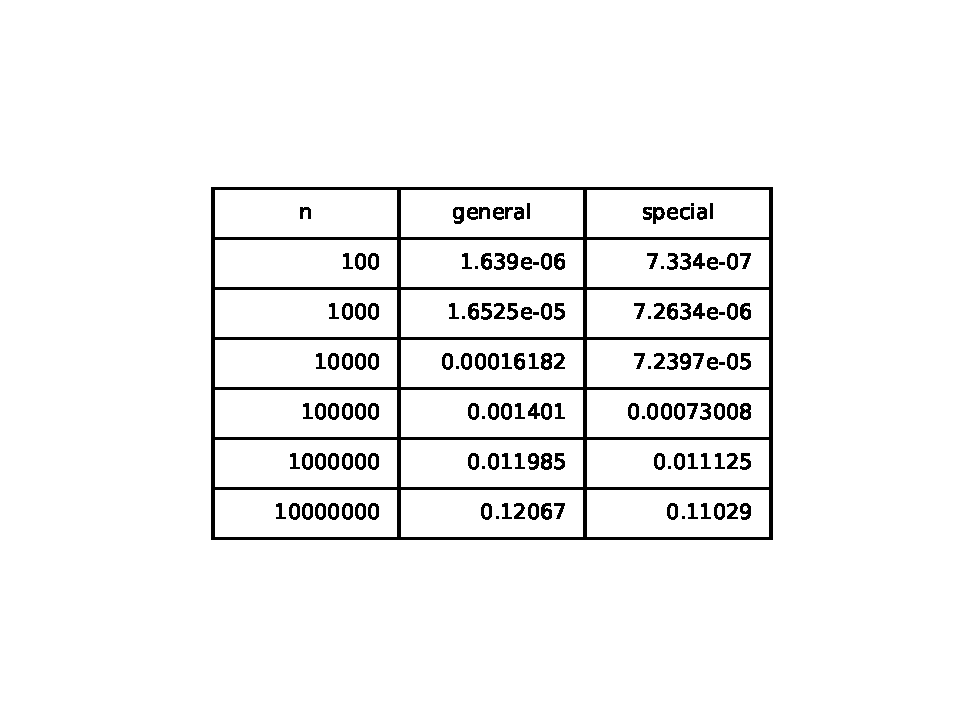
\includegraphics[scale=0.75]{plots/cmp_gen_spec.pdf} %Imports the figure.
		\caption{A table showing the running time of the general and special algorithm for a given $n$}
		\label{fig:cmp_gen_spec}
	\end{figure}
By pure FLOP count the special should be about 25\% faster, but we're not seeing quite that big gains. There are some outliers, but it is probably safe to assume that is due to some of the data being in cache. Assuming loading from memory is the bottleneck the speed up could also be due to the special algorithm loading less data.

\section*{problem 11}
LU decomposition has a complexity of $O(N^3) (+O(N^2))$ vs our algorithm that runs in $O(N)$. for $n=10^5$ I would expect to: \\
\begin{enumerate}
	\item Run out of memory, since you need to store $8*N*N = 8*10^5*10^5 = 8*10^{10} \approx 80$GB.
	\item To be very slow. The alogrithm's $O$ factor is two orders of magnitude larger, so probably around 100 times as long.
\end{enumerate}

\end{document}